\chapter{THEORETICAL BACKGROUND}
\section{Interaction of photons or $\gamma$-quanta with matter}
\subsection*{Photoelectric effect}
The \textit{photoelectric effect} describes the effect of a $\gamma$-quantum interacting with matter. If the energy of the photon $\mathit{E_{\gamma}=h\nu}$ is higher than the electron binding energy (the work function) of the material, the electron is ejected. If the energy is too low the electron is not able to escape. In case of the ejection the electron has the energy $\mathit{E_{e^{-}}=h\nu-E_{D}}$ and leaves a free place in the electron shell. Because of the lower energy an electron of a higher shell falls down in that free spot by emitting a photon or an Auger-electron. The cross-section of the \textit{photoelectric effect} is defined as $\mathit{\rho_{photo}\propto Z^{5}/E^{\frac{7}{2}}}$.

\subsection*{Compton scattering}
If a $\gamma$-quantum hits an outer or a free electron and they perform an inelastic scattering so that the $\gamma$-quantum gives a part of its energy to the electron, it is called \textit{Compton Scattering}. The deflection angle $\theta$ depends on the energy of the $\gamma$-quantum. The probability of this effect taking place increases with the atomic number $\mathit{Z}$ of the absorbing material as well as at an energy of 200 keV to 5 MeV.

\subsection*{Pair production}
At an energy of 1.022 MeV and above there is another effect, the \textit{Pair production}. At that point the energy of the $\gamma$-quantum is as high as the energy of a positron-electron-pair at zero velocity. So a pair of these could be excited in the field of an electron or an nucleus. The free positron annihilates when reaching the surrounding matter by sending out two $\gamma$-quanta with energy of 0.511 MeV per quantum.

\section{Interference of photons}
As is known there could be interference effects with photons for example when photons pass through a grid. That effect could also be  appearing with single photons, as is known from quantum physics.

\section{Semiconductor and single-element semiconductor}
\textit{Semiconductor} are materials whose conductivity or rather electrical resistance is related to a parameter which depends on the temperature. \textit{single-element semiconductor} are \textit{semiconductor} out of one single material; for example germanium or silicon.

\section{Band structure}
The \textit{Band structure} is a model of quantum physics and helps to distinguish between conductor, semiconductor and insulator. In that model we use an energy level called valence band where the electrons normally are and a higher energy level called the conduction band. The energy difference between these two bands is the bandgap. In a conductor the energy level of valence and conduction band crosses partly or completely so there is no band gap. In a semiconductor the electron can cross the band gap by getting energy and in an insulator the bandgap is normally too big for an electron to cross it.\\
\begin{figure}[h]
\begin{center}
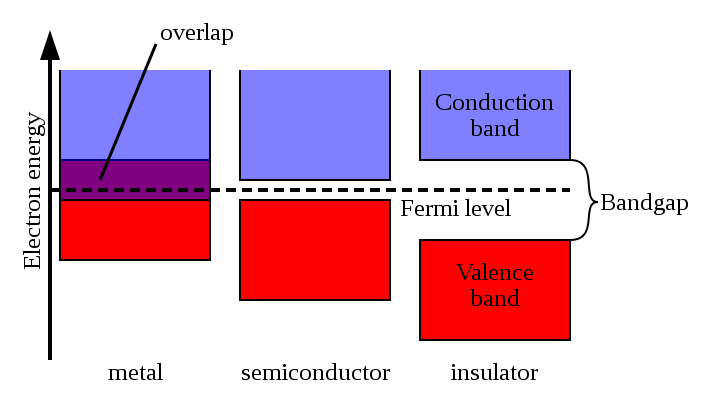
\includegraphics[scale=0.3]{bilder/isolator-metal}
\caption{ Band structure of a conductor, semiconductor and insulator. Source:[sclo] }
\label{fig:band}
\end{center}
\end{figure}
\\
A semi-classical way to describe the model: You can observe two atoms which are placed far away from each other. Their electrons have discrete levels of energy. If you decrease the distance between these electrons that leads to an interaction and the wave-functions of those electrons overlap. The Pauli exclusion principle gives us now a separation in two
\begin{figure}[h]
\begin{center}
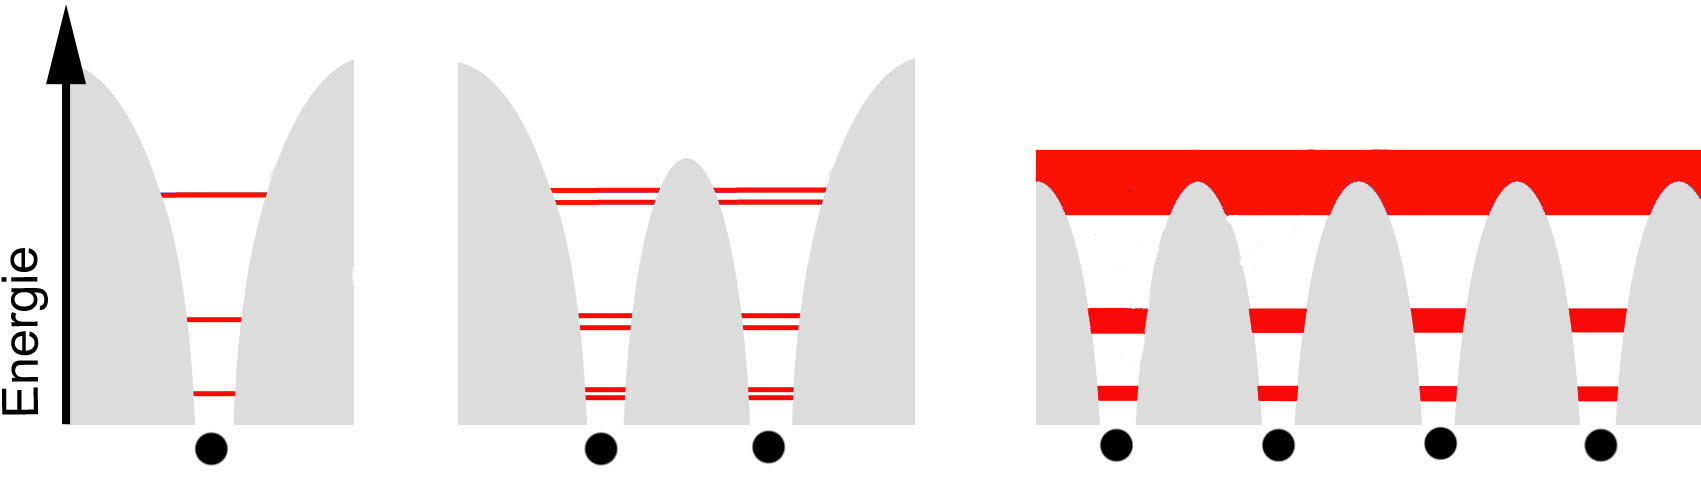
\includegraphics[scale=0.2]{bilder/energieniveaus-pauli}
\caption{Energy levels of: 1.single atom, 2.two atoms, 3.solid state body. Source:[Amr] }
\label{fig:pauli}
\end{center}
\end{figure}
\\
slightly separated energy levels, what leads, because of the high count of electrons, to continuous energy bands.
\section{Charge carrier in semiconductor}
If an electron moves to the conduction band it leaves a free spot in the valence band. That spot can be seen as an positive charge carrier. So there are negative electron and positive charge carriers in a semiconductor. If an external voltage is applied, the electrons move in the direction of the positive pole and the free spots in the direction of the negative pole.
\begin{figure}[h]
\begin{center}
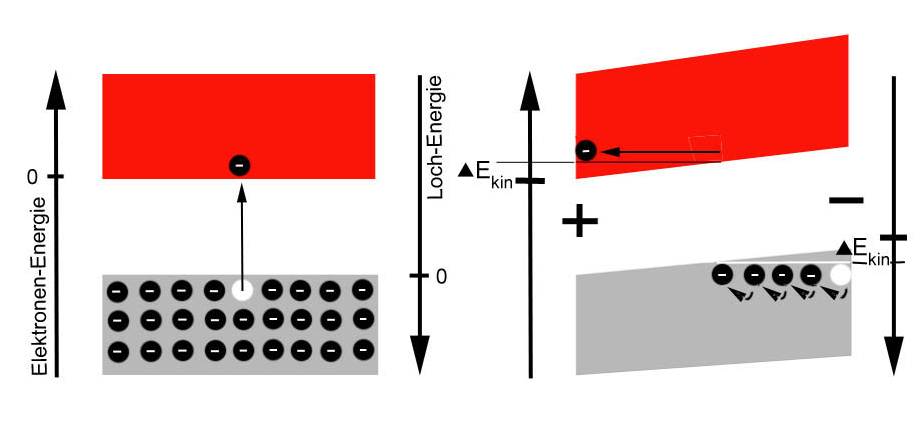
\includegraphics[scale=0.3]{bilder/ladungstraeger}
\caption{Band crossing (left) and external voltage (right). Source:[Amr] }
\label{fig:ladungs}
\end{center}
\end{figure}
\\
\section{Exponential decay and mean lifetime}
The time between the appearance of an electron-spot-pair and its recombination is called mean lifetime. If you now look at a lot of these events, you can describe the count of the not yet recombined pairs $\mathit{N(t)}$ after a time interval $\mathit{t}$ as an exponential decay:
\begin{center}
$\mathit{N(t)=N_{0}\cdot e^{-t/\tau}}$
\end{center}
Where $mathit{N_{0}}$ is the count of pairs at $mathit{t=0}$ and $mathi{\tau}$ is the average lifetime. If there is an external voltage, the average lifetime is now important to calculate the average velocity of the charge carrier:
\begin{center}
$\mathit{\vec{v}_{p/n}=\pm\frac{e\tau}{m_{p/n}}\vec{E}=\pm\mu_{p/n}\vec{E}}$
\end{center}
$\mathit{p/n}$ is the type of the charge, $\mathit{m}$ is the mass of the charge carrier an $\mathit{\mu}$ the mobility of the carrier.
\section{Direct and indirect semiconductor}
In the wavenumber space we can observe the energy in relation to its wavenumber. The upper line of the valence band and the bottom line of the conduction band are now no longer parallel. You can now differentiate between the direct semiconductor where the maximum of the valence band lies directly under the minimum of the conduction band and the indirect semiconductor where that extrema are shifted by  $\mathit{\delta\vec{p}}$.
\begin{figure}[h]
\begin{center}
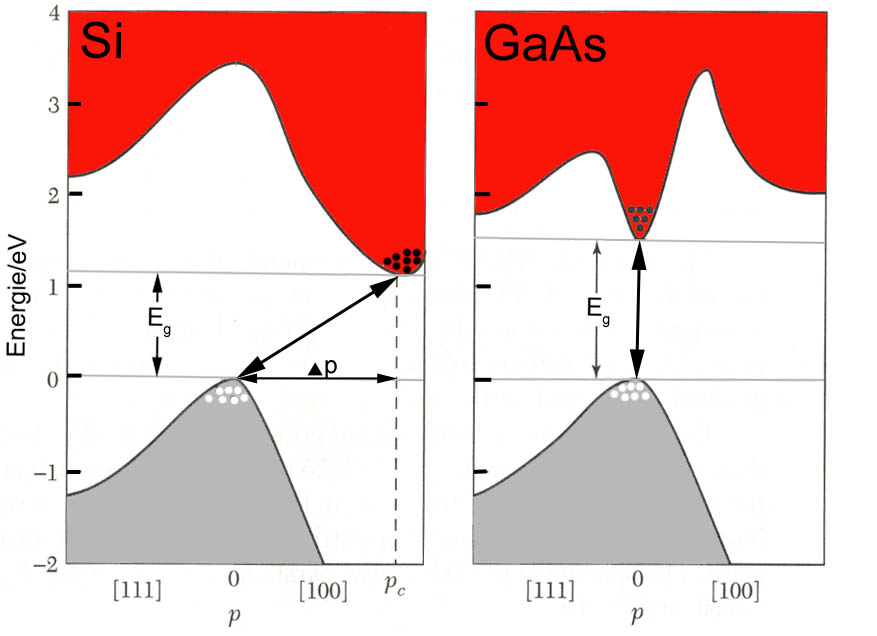
\includegraphics[scale=0.3]{bilder/impulsraum}
\caption{indirect semiconductor (left) and direct semiconductor (right). Source:[Amr] }
\label{fig:impuls}
\end{center}
\end{figure}
\\
\section{Intrinsic and extrinsic semiconductor, Doping}
\textit{Intrinsic semiconductor} are semiconductors with a perfect crystal structure without any errors or contamination. It is not possible to create crystals like these. Real semiconductors have contaminations and defects in the structure. At the structure of the crystal there could be parts of the structure defect or displaced. Because of that, there could be new band levels and the band gap could be distorted. Foreign atoms could also cause errors.
\subsection*{Doping}
Volitional contamination with atoms with more or less valence electrons as the atoms of the crystal is called \textit{doping}. A foreign atom with an electron more is called a \textit{donor} and one with an electron less is called \textit{acceptor}. Additional electrons are not implemented in the crystal structure and can be seen as free electrons for the conduction band. Missing electrons are free spots and can be seen as free positive charge carriers.\\
The contamination with donors is a p-doping and with acceptors is a n-doping. The specific conductivity could grow by doping a semiconductor.
\section{p-n-Diode, Use as semiconductor detector}
If you put a p-doped and an n-doped together (in contact) free electrons diffuse from the n-layer in the free spots in the p-layer at the contact area. Because of that, the free charges get balanced out in that area. The kernel can't get out of the crystal structure, so after that balancing there are positive kernels left in the n-doped layer and negative kernels left in the p-doped layer, whereby an electric field develop in that area. This is called contact electrification with the voltage $\mathit{U_{bi}}$.\\
Is a charge generated by an outer stimulation, generated charges will be accelerated and leave the depletion layer. For the usage as a semiconductor detector you can use such a diode. If a photon passes the depletion layer, an electric current will be generated because of the photo- or Compton-effect.
\begin{figure}[h]
\begin{center}
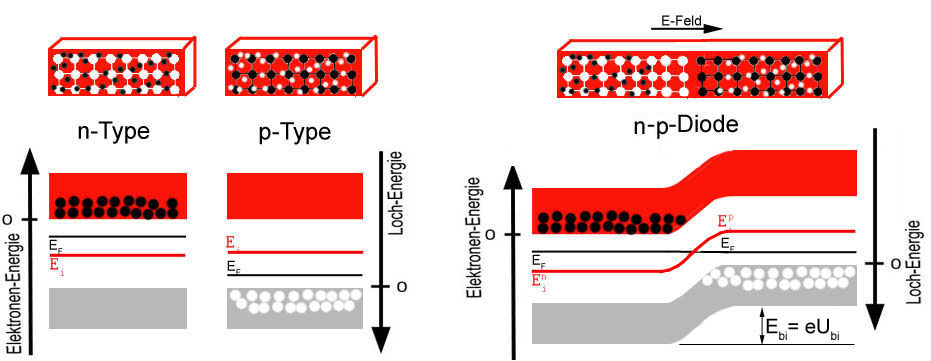
\includegraphics[scale=0.5]{bilder/diode}
\caption{Semiconductor layer (left), diode (right). Source:[Amr] }
\label{fig:diode}
\end{center}
\end{figure}
\section{Electronics}
\subsection*{Preamplifier}
Preamplifiers cause a linear amplification of electric signals in detectors and other, similar electronic devices. Often these amplifiers are built-in.\\
\subsection*{Shaping Amplifier}
A shaping amplifier is an electronic amplifier which can shape the incoming signal. In this experiment, a $(CR)-(RC)^2$-SA is used. 
\subsection*{Multi Channel Analyzer}
An MCA is applied to record electronic signals of different voltage. It consists of many channels, which are connected to voltages linearly. This way incoming signals are matched with the appropriate channel.
\subsection*{Lock-In Amplifier}
The lock-in method is used to visualize weak signals in heavy noise. The incoming and a reference signal are applied to a synchron detector. The signals are multiplied, integrated with the help of a low-pass and eventually amplified. This way only the part of the incoming signal which has the same frequency and phase as the reference signal is let through.
